\section{Možnosti riešenia špecifických úloh}\label{sec:algorithms}
Riešením je teda algoritmus, ktorý je protihráčom v hre piškvorky hranej v trojrozmernom hracom priestore v prostredí
Cave.
Počas vývoja výpočtovej techniky sa vyvíjali algoritmy aj pre kombinatorické hry, pričom piškvorky sú jednou z nich.
Tieto algoritmy je možné rozdeliť do 2 skupín: \emph{exaktné} a \emph{heuristické}; v tejto kapitole je popísaný jeden
algoritmus z každej skupiny.

\subsection{MiniMax}\label{subsec:algo-minmax}

Minimax je rozhodovacie pravidlo založené na vyhľadávacom algoritme v strome, podľa ktorého je možné určiť nasledujúci
ťah.\cite{algo_minimax}
Jeho princíp spočíva v maximalizovaní úžitku pre cieľového hráča a minimalizovaní úžitku pre oponenta.
Pôvodne bol vyvinutý pre \emph{hru s nulovým súčtom} (angl. zero-sum), čo je termín používaný v teórii hier.
Vyjadruje hru, kde rozhodnutia hráčov sa dajú ohodnotiť kladným nenulovým číslom $v$, pričom súčet za sebou idúcich hier
má súčet približne 0.
Často používaná hodnota je $v=1$ alebo $v=10$.
Ťah cieľového hráča je vyjadrený kladnou hodnotou ($+v$), ťah protihráča je vyjadrený zápornou hodnotou ($-v$) a remíza
je vyjadrená hodnotou $0$.
Hru, ktorú hrajú hráči striedavo, je možné vyjadriť pomocou postupnosti pre remízu:
\begin{equation}
    v-v+v-v+ \dots = \sum{v-v} = \sum{0} = 0
\end{equation}
(z čoho vychádza aj názov \emph{hra s nulovým súčtom}), resp. pre výhru jedného z hráčov:
\begin{equation}
    \pm v+v-v+v-v+ \dots = \pm v+\sum{v-v} = \pm v+\sum{0} = \pm v
\end{equation}
Rozhodovanie vychádza práve z tohto faktu, pričom algoritmus sa snaží nájsť takú postupnosť ťahov, ktorá by bola rovná
$\max\{-v, 0, +v\}$ (resp. maximálna), čo by znamenalo výhru cieľového hráča, v horšom prípade remízu a v tom najhoršom
prípade prehru cieľového hráča.
Samotný rozhodovací proces sa dá vyjadriť pomocou rozhodovacieho stromu vychádzajúceho z ktoréhokoľvek stavu hry.
Stav hry sa dá vyjadriť pomocou $d$-rozmernej tabuľky, kde hodnoty predstavujú \textbf{X}, \textbf{O} alebo prázdne
políčko.
Stavy hry tvoria vrcholy stromu a hrany predstavujú prechody medzi týmito stavmi.

Nech $l$ je maximálna výška rozhodovacieho stromu.
Ak nie je explicitne zadaná, potom maximálna výška stromu je počet voľných políčok vo východiskovom stave hry.
Nech $S_{ij}$ je stav hry, kde $i$ je úroveň stromu, v ktorom sa stav hry nachádza a $j$ je poradové číslo tohto vrcholu
v rámci úrovne $i$ určené pre jednoznačnú identifikáciu stavu hry a nech $p(S_{ij})$ je v strome rodič stavu $S_{ij}$
potom $\forall i, k, j \colon p(S_{i+1,k}) = S_{ij} \colon S_{i+1,k}$ vznikne vyplnením postupne každého
prázdneho políčka znakom hráča, ktorý je na ťahu na úrovni $i$.

Pre lepšiu predstavu je možné si situáciu ukázať na príklade z \hyperref[figure:minimax-tree]{nasledujúceho obrázku}.
Koreň stromu obsahuje 3 voľné políčka, jeho synovia vzniknú vyplnením postupne každého voľného políčka znakom hráča na
úrovni 2 (tzn. \textbf{X}: na pozície 1. riadok, druhý stĺpec; tretí riadok, prvý stĺpec a tretí riadok, tretí stĺpec).
Takto sa naplní celý strom a jeho listy sa ohodnotia hotnotami $v$ pre víťazný stav hry, $-v$ pre prehru a $0$ pre
remízu (na \hyperref[figure:minimax-tree]{obrázku} vyznačené čiernou farbou).

Nech
\begin{equation}
    V(S_{ij}) =
    \begin{cases}
        \min{\{V(S_{i+1,j}) \forall j\}} & \text{ak v ťahu } i \text{ je na ťahu protihráč} \\
        \max{\{V(S_{i+1,j}) \forall j\}} & \text{ak v ťahu } i \text{ je na ťahu cieľový hráč}
    \end{cases}
\end{equation}
potom $\forall S_{ij}$ je priradená hodnota $V(S_{ij})$ pre $i = 1 \dots l-1$ a $\forall j$.
Najlepší ťah je potom určený spôsobom
\begin{equation}
    S_{Best} = \max{\{V(S_{2j}) \forall j \colon p(S_{2j}) = S_{11}\}} = \max{\{V(S_{2j}) \forall j\}}
\end{equation}
Vyhľadávanie prebieha potom nasledovne:\cite{algo_minimax_pseudocode}
\begin{tiny}
    \begin{lstlisting}[
      mathescape,
      columns=fullflexible,
      escapeinside={(@}{@)},
      basicstyle=\fontfamily{lmvtt}\selectfont,
    ]
def minimax(hraciaPlocha, int maximalnaHlbka, bool maximalizacia):
    if maximalnaHlbka = 0 or hraciaPlocha (@ nem\'{a} \v{z}iaden dostupn\'{y} mo\v{z}n\'{y} \v{t}ah @):
        return hodnota hracej plochy
    if maximalizacia:
        najlepsiaHodnota = -$\infty$
        for (@ v\v{s}etky dostupné \v{t}ahy v hracej ploche @):
            novaHraciaPlocha = (@ vykonaj \v{t}ah v hraciaPlocha @)
            aktualnaHodnota, aktualnyTah = minimax(novaHraciaPlocha, maximalnaHlbka - 1, false))
            if aktualnaHodnota > najlepsiaHodnota:
                najlepsiaHodnota := aktualnaHodnota
                najlepsiTah = aktualnyTah
        return najlepsiaHodnota, najlepsiTah
    else:
        najlepsiaHodnota = $\infty$
        for (@ v\v{s}etky dostupné \v{t}ahy v hracej ploche @):
            novaHraciaPlocha = (@ vykonaj \v{t}ah v hraciaPlocha @)
            aktualnaHodnota, aktualnyTah = minimax(novaHraciaPlocha, maximalnaHlbka - 1, true))
            if aktualnaHodnota < najlepsiaHodnota:
                najlepsiaHodnota := aktualnaHodnota
                najlepsiTah = aktualnyTah
        return najlepsiaHodnota, najlepsiTah
\end{lstlisting}
\end{tiny}

\begin{figure}[H]
    \centering
    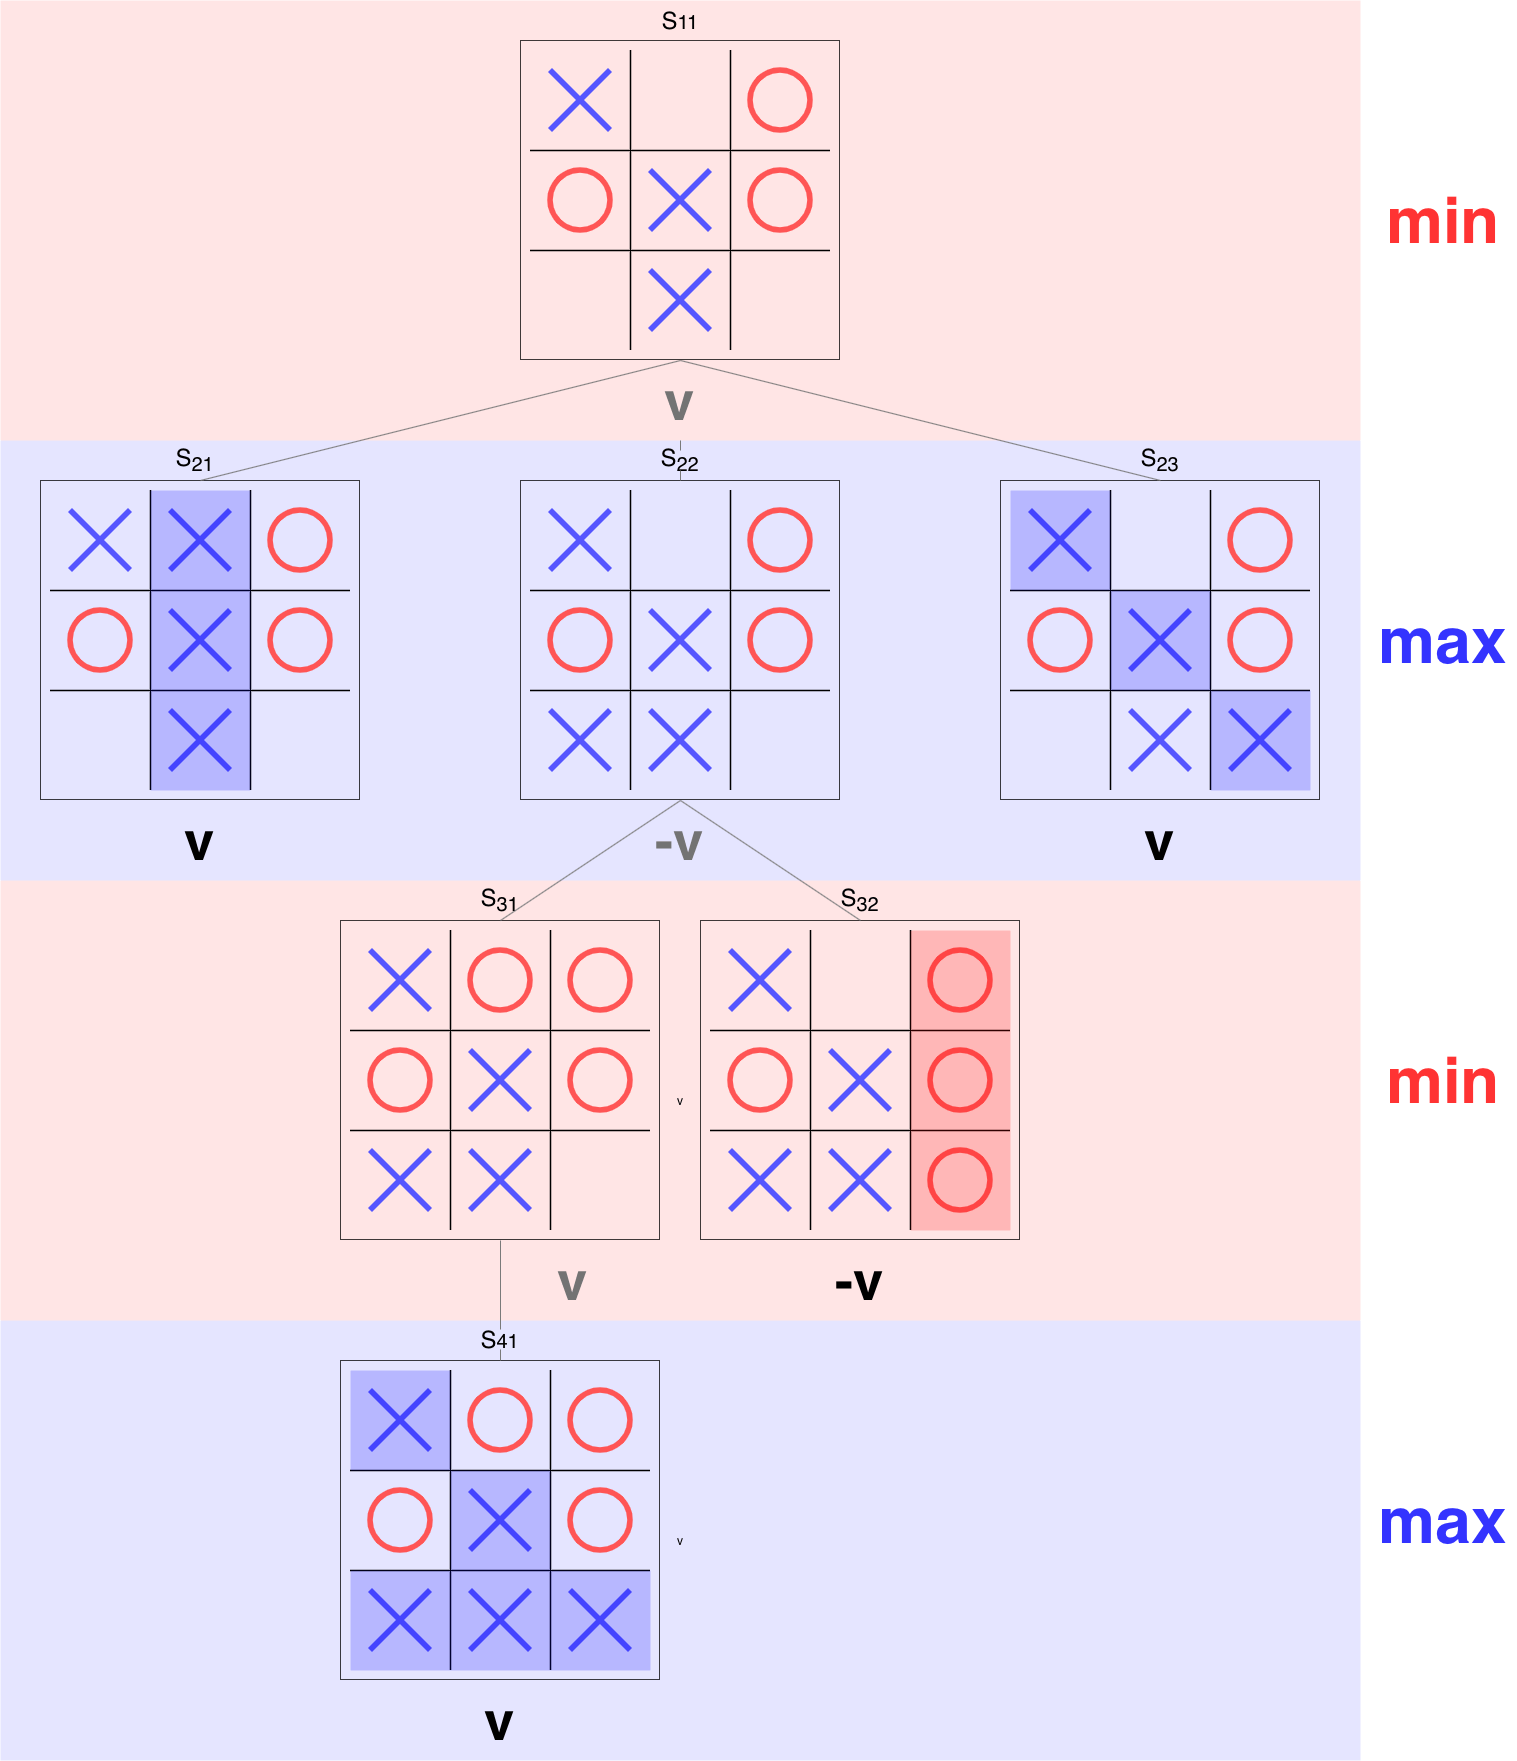
\includegraphics[width=0.8\textwidth]{images/minmax-tree.png}
    \caption{Rozhodovací strom algoritmu Minimax}
\end{figure}\label{figure:minimax-tree}

Algoritmus minimax patrí medzi \emph{exaktné algoritmy}, čo znamená, že pri hľadaní nájde najlepšie (optimálne)
riešenie, no prehľadáva všetky možné riešenia (celý priestor riešení).
Vo všeobecnosti pre neprázdne hracie pole o veľkosti $r$ v $d$-rozmernom hracom priestore s $o$ obsadenými políčkami je
možné veľkosť celého priestoru riešení vypočítať ako
\begin{equation}
    C(r, d, o) = (r^d - o) * (r^d - o - 1) * (r^d - o - 2) \dots 1 = \prod_{i = 1}^{r^d - o}{(r^d - o - i + 1)}
\end{equation}
Pre prázdne hracie pole (teda, kde $o = 0$) platí
\begin{equation}
    C(r, d, 0) = (r^d) * (r^d - 1) * (r^d - 2) \dots 1 = \prod_{i = 1}^{r^d}{(r^d - i + 1)}
\end{equation}

Ak algoritmus vychádza z prázdneho poľa o veľkosti $3 \times 3$ ($r = 3$, $d = 2$) je veľkosť priestoru riešení
$\prod_{i = 1}^{9}{(10 - i)} =$ \textbf{362 880}.
Na preskúmanie takéhoto počtu je možné použiť aj komerčnú výpočtovú techniku pričom výsledok bude známy v čase menšom
ako jedna minúta, no pri veľkosti $4 \times 4$ (teda $r = 4$, $d = 2$) je $C(4, 2, 0) \approx 2*10^{13}$ a čas
prehľadania priestoru sa (za predpokladu, že preskúmanie 1 možnosti trvá 1 milisekundu) zvýši na
\emph{$\approx 663$ rokov}.
Pre trojrozmernú plochu s rozmerom $3$ ($r = 3$, $d = 3$) je $C(3, 3, 0) \approx 1.08 * 10^{28}$, čo s rovnakým časovým
predpokladom znamená, že takýto výpočet by sa skončil po $\approx 3*10^{17}$ rokoch (pre predstavu: vek vesmíru sa
odhaduje na $\approx 14$ mld. $\approx 14 * 10^9$ rokov).

\subsection{Umelá neurónová sieť}\label{subsec:algo-ann}

Z vyššie uvedeného vyplýva, že exaktné riešenie pre väčšie rozmery plochy nie je možné použiť, teda je nutné použiť
algoritmy, ktoré nenájdu najlepšie riešenie v rámci celého priestoru riešení (optimálne), no vedia nájsť
najlepšie riešenie v rámci obmedzeného priestoru riešení (suboptimálne).
Jednou z týchto heuristických metód je \emph{umelá neurónová sieť} angl. artificial neural network
(často označovaná ako ANN).

Matematické základy pre tento algoritmus boli vytvorené už v polovici 20. storočia a sú založené na modeli
biologických neurónových sietí, z čoho vychádza aj názov a terminológia.\cite{algo_ann_history}
Sieť pozostáva z \textbf{vrstiev}, ktoré sú tvorené \textbf{neurónmi}.
Medzi jednotlivými neurónmi sú prepojenia nazývané tiež \textbf{synapsy}.\cite{algo_ann_terminology}
Umelú neurónovú sieť je možné reprezentovať ohodnoteným \hyperref[figure:general-ann]{grafom}, kde vrcholy reprezentujú
neuróny a hrany synaptické spojenia.
Graf môže vyzerať nasledovne:
\begin{figure}[H]
    \centering
    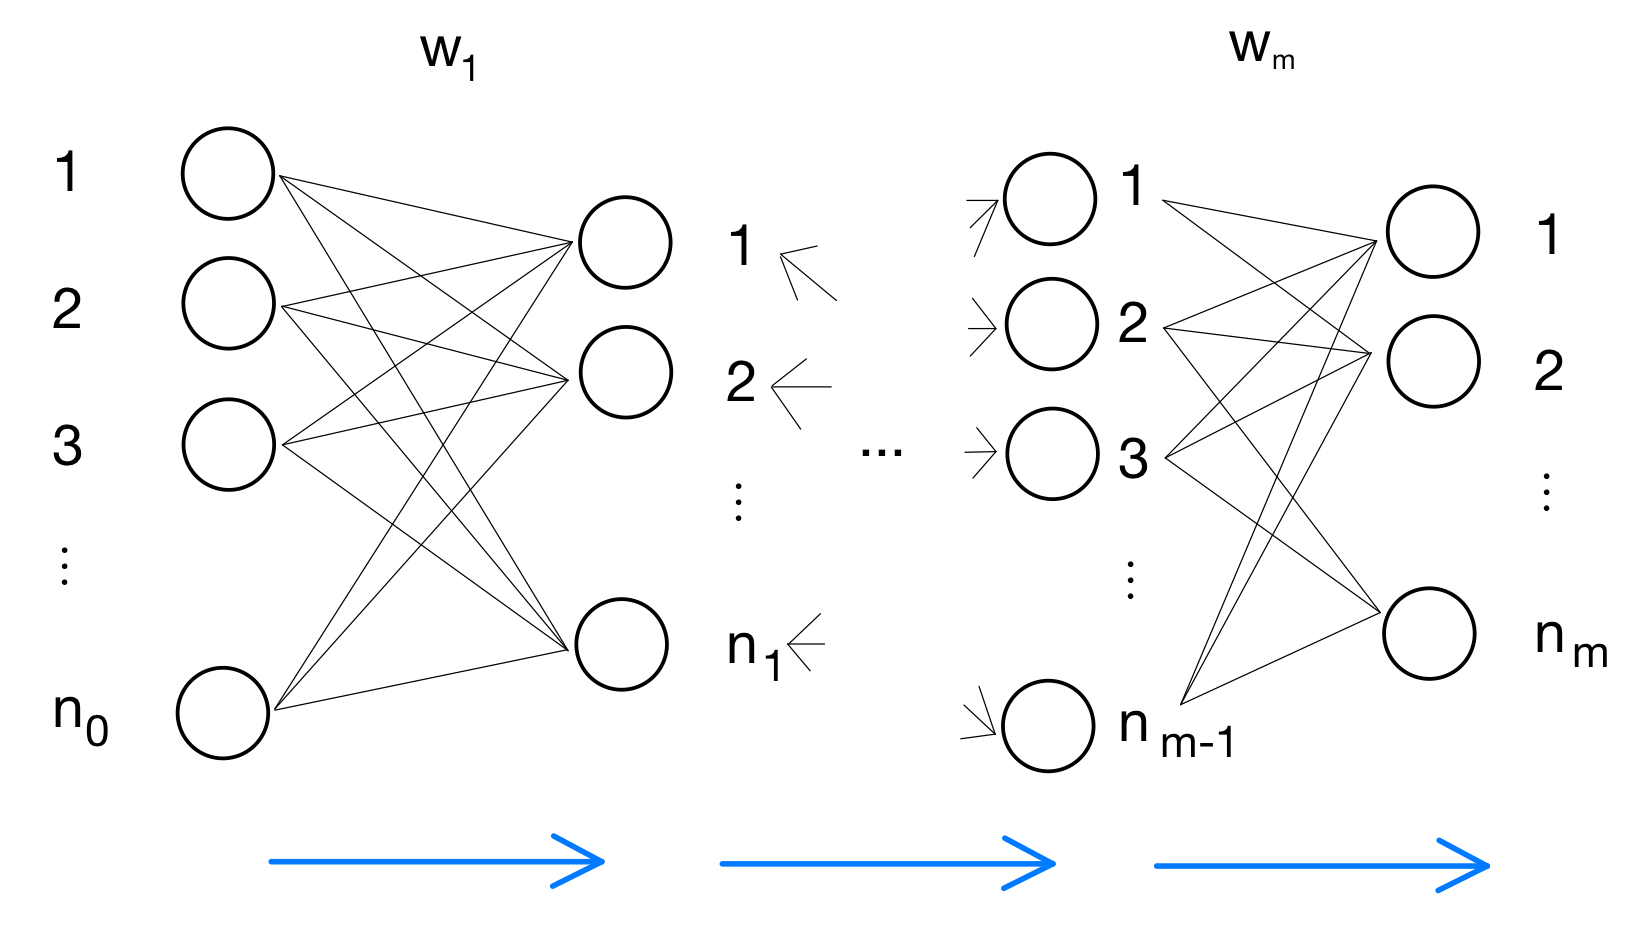
\includegraphics[width=0.5\textwidth]{images/general-ann.jpg}
    \caption{Všeobecná dopredná umelá neurónová sieť}
\end{figure}\label{figure:general-ann}
Nech $m$ je počet vrstiev v umelej neurónovej sieti a $n_i$ pre $i = 0 \dots m$ je počet neurónov vo vrstve $i$.
Existuje mnoho typov umelých neurónových sietí, no všeobecne sa ako ANN označuje dopredná umelá neurónová sieť (
angl. feed forward neural network, skr. FFNN).
V doprednej umelej neurónovej sieti existujú synapsy (spojenia) len medzi vrstvami $i$ a $i + 1$ pre
$i = 0 \dots m - 1$, tzn. spojenia existujú len medzi za sebou idúcimi vrstvami smerom od vstupnej ($i=0$) k výstupnej
($i=m$) vrstve.

Každému neurónu je priradená aktivačná funkcia.
Z biologického hľadiska vyjadruje akčný potenciál bunky a teda potenciálny prenos informácie cez synaptické prepojenie.
V rámci umelých neurónových sietí aktivačná funkcia vyjadruje to isté: je to binárna funkcia a neurón sa aktivuje
ak na výstupe z tejto funkcie je 1.
Aktivačná funkcia závisí od vstupov predchádzajúcich neurónov.
Nech $N_{ij}$ pre $i = 1 \dots m-1$, $j = 1 \dots n_i$ je $j$-ty neurón v $i$-tej vrstve.
Na vstup do tohto neurónu sa z predchádzajúcej vrstvy prenesú informácie vo vektore $\pmb{x_{ij}}$.
$\forall h \in \pmb{x_{ij}} \colon h \in \{0, 1\}$.
Pre všetky synaptické spojenia existujú tzv. \emph{váhy}, ktoré zosilňujú (resp. zoslabujú) účinok signálu z
predchádzajúcich neurónov.
Nech $w_{ijk}$ pre $i=1 \dots m$, $k=1 \dots n_{i-1}$, $j=1 \dots n_i$ je váha pre synaptické spojenie vedúce z
neurónu $k$ vo vrstve $i-1$ k neurónu $j$ vo vrstve $i$ resp.
nech vektor $\pmb{w_{ij}}$ je vektor váh definovaných pre neurón $N_{ij}$ a nech
\begin{equation}
    z = \sum_{k=1}^{|\pmb{w_{ij}}|=|\pmb{x_{ij}}|}{w_{ijk} * x_{ijk}}-\theta
\end{equation}
kde $\theta$ je tiež označovaná ako prahová hodnota (angl. threshold).
\hyperref[figure:activation-functions]{Aktivačná funkcia} sa označuje ako $\phi(z)$.
Medzi bežne používané aktivačné funkcie patrí napríklad:
\linebreak
\textbf{SoftMax} (táto aktivačná funkcia sa využíva pri kategorizácii)\cite{algo_ann_activation_softmax}
\begin{equation}
    \phi(\mathbf{z})_i = \frac{e^{z_i}}{\sum_{j=1}^{|z|}{e^{z_j}}}
\end{equation}
\textbf{Sigmoid}\cite{algo_ann_activation_sigmoid}
\begin{equation}
    \phi(z) = \frac{1}{1+e^{-z}}
\end{equation}
\textbf{Hyperbolická funkcia}\cite{algo_ann_activation_hyperbolic}
\begin{equation}
    \phi(z) = tanh(z)
\end{equation}
\textbf{ReLu}\cite{algo_ann_activation_relu}
\begin{equation}
    \phi(z) = \max\{0, x\}
\end{equation}

Priebehy niektorých týchto funkcií sú zobrazené na grafe.
\begin{figure}[H]
    \centering
    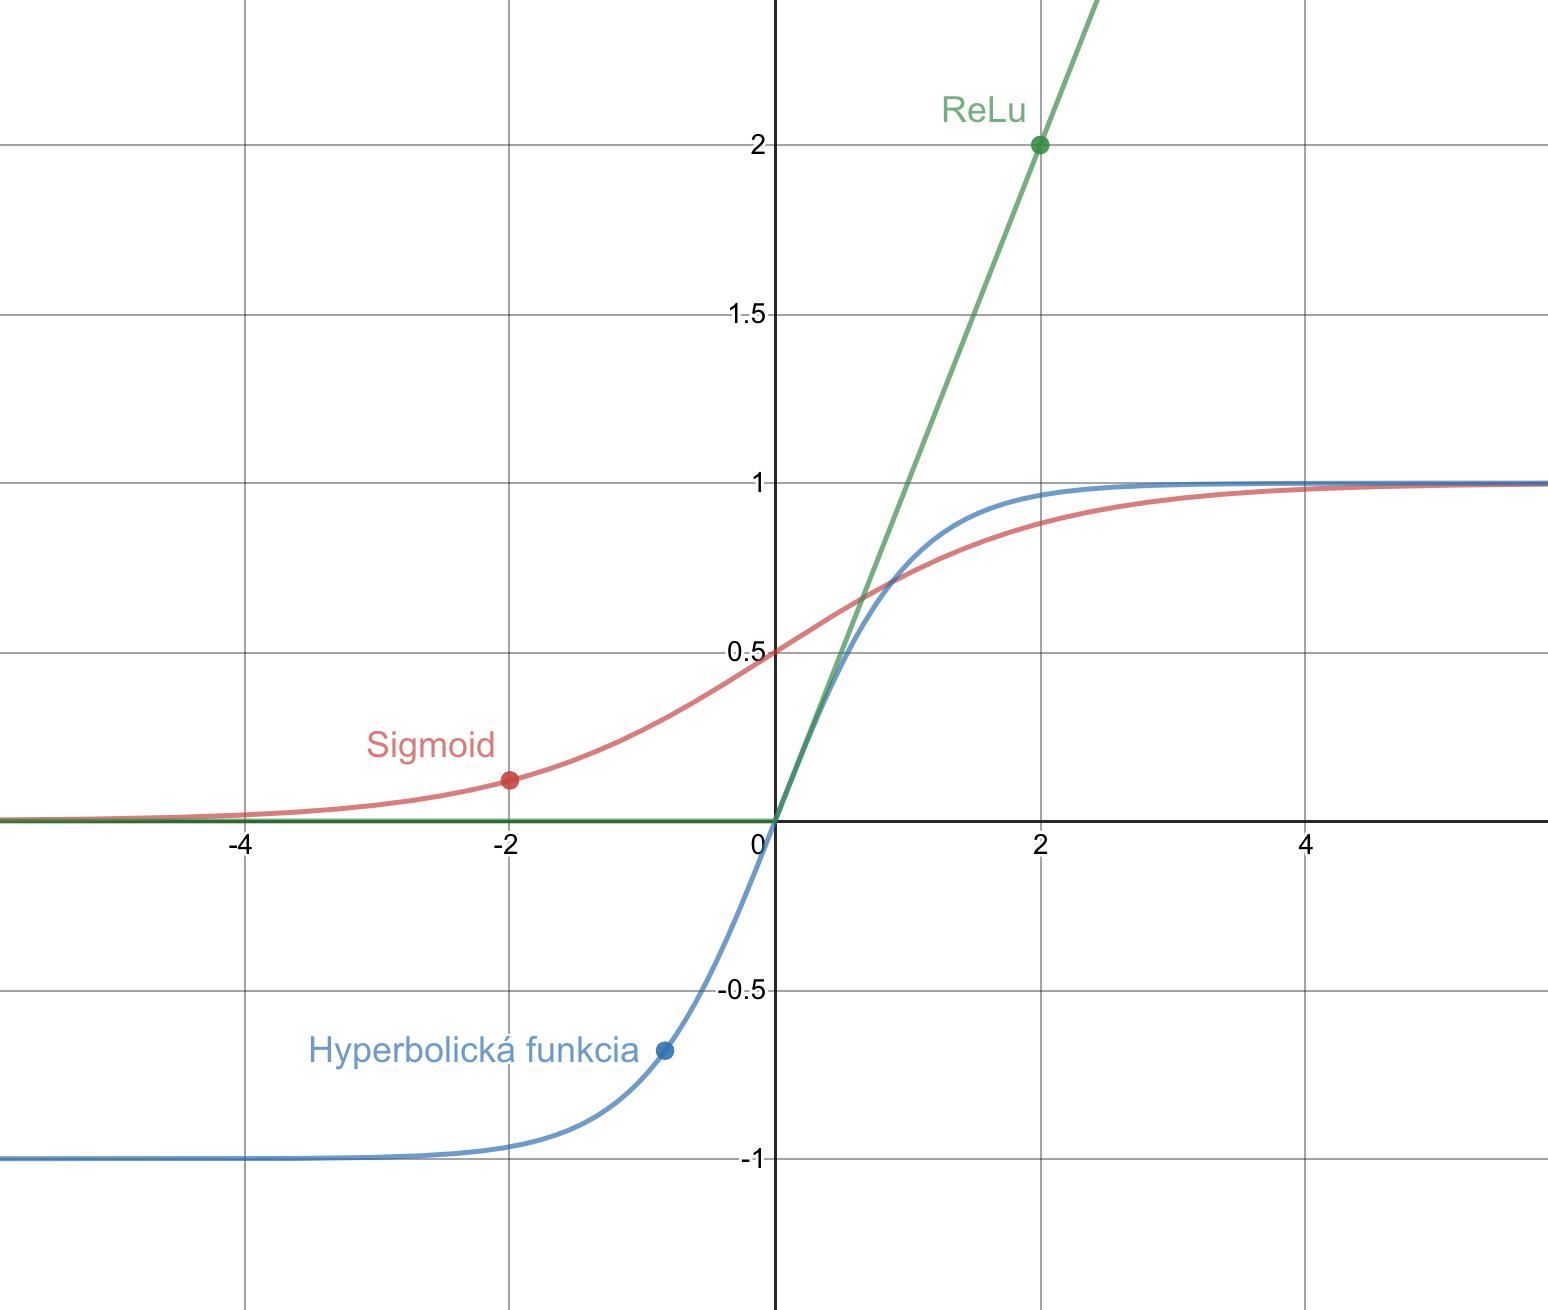
\includegraphics[width=0.8\textwidth]{images/activation-functions.png}
    \caption{Priebehy aktivačných funkcií}
\end{figure}\label{figure:activation-functions}

Pri vytváraní umelej neurónovej siete je potrebné dbať na jej správnu štruktúru a nastavenie váh.
Váhy sa dajú nastaviť tzv. učením siete.
Učenie prebieha v 2 fázach: trénovanie a testovanie siete.
V prvej fáze sa sieť naplní \emph{existujúcimi} vstupmi a výstupmi, aby vedela odhadnúť vzťah medzi nimi.
Existuje mnoho tréningových metód, no v tejto práci sú popísané 2:
\begin{itemize}
    \item algoritmus založený na delta prístupe\cite{algo_ann_delta_rule}
    \item algoritmus založený na spätnom šírení\cite{algo_ann_backpropagation}
\end{itemize}
Pri oboch prístupoch je nutné definovať tzv. trénovaciu ($T_r$) a testovaciu množinu ($T_t$).
Trénovacia množina slúži na prvotné nastavenie parametrov (váh).
Využíva sa vo fáze trénovania.
Natrénovaná sieť sa v druhej fáze otestuje pomocou testovacej množiny.

Pri \textbf{algoritme založenom na delta prístupe} (ďalej len delta algoritmus) sa pracuje len s dvojvrstvovou
umelou neurónovou sieťou, resp. s vrstvou, ktorá ma len jednu sadu synaptických prepojení.
Princíp spočíva v postupnom vyhodnocovaní rozdielu medzi výstupom z umelej neurónovej siete pri určitom vstupe
(reálny výstup - angl. actual) a správnym výstupom (očakávaný výstup - angl. expected).
Parametre ANN sú upravované v závislosti od tohto rozdielu.

Nech $\gamma \in (0, \infty)$ je učiaci parameter, $\epsilon$ je maximálny akceptovateľný rozdiel v hodnotách reálneho
a očakávaného výstupu a $s$ je počet za sebou idúcich rozdielov výstupov (rozdiel nemusí byť vyhodnocovaný len
prostredníctvom absolútnej hodnoty, často sa využíva aj druhá mocnina rozdielu), ktoré sa nachádzali v intervale
$<0, \epsilon>$.
Ďalej nech $|T_r|$ je veľkosť trénovacej množiny (teda počet vzoriek), $\mathbf{X_i}$ pre $i=1 \dots |T_r|$ je vzorka
z trénovacej množiny, ktorej je pridelený očakávaný výstup $y_i$ pre $i=1 \dots |T_r|$ a nech $y(\mathbf{X_i})$ je reálny
výstup siete ako odpoveď na vstup $\mathbf{X_i}$.
Algoritmus prebieha nasledovne:\cite{algo_ann_delta_rule}
\begin{enumerate}
    \item Inicializácia počiatočných váh $\pmb{w_1}$, prahovej hodnoty $\theta$ a parametrov $\gamma$, $\epsilon$ a $s$.
    \item pre $i = 1 \dots |T_r|$:
    \begin{enumerate}
        \item ak $(y_i-y(\mathbf{X_i}))^2>\epsilon$: \\
                $\Delta{w_j} = \gamma * (y_i-y(\mathbf{X_i}))_j$ \\
                $\pmb{w_{1j}}=\pmb{w_{1j}} + \Delta{w_j} * X_{ij}$ \\
                $\theta=\theta + \Delta{w_j}$
        \item ak prebehlo $s$ za sebou idúcich rozdielov výstupov, ktoré sa nachádzali v rámci $\epsilon$, tak koniec
    \end{enumerate}
\end{enumerate}
Zmena váh o vektor $\Delta (y_i-y(\mathbf{X_i}))$ vyzerá ako intuitívne riešenie, no je možné si ukázať, že to funguje
aj matematicky.
Nech $\pmb{\omega_0}$ je východiskový bod pre váhy a nech $f(\pmb{x})$ je funkcia vyjadrujúca mieru chyby v sieti,
ktorú je potreba minimalizovať.
K bodu $\pmb{\omega_1}$ je možné sa z východiskového bodu posunúť v jednotkovom smere $\pmb{d}$ ($|\pmb{d}|=1$) o krok
dĺžky $\alpha$, tzn.
\begin{equation}
    \pmb{\omega_1} = \pmb{\omega_0} + \alpha\pmb{d}
\end{equation}
Tu je nutné vyriešiť problém, ako zvoliť veľkosť kroku $\alpha$, tak aby $f(\pmb{\omega_1}) < f(\pmb{\omega_0})$.
Riešením tohto problému je \textbf{derivácia} funkcie, ktorá vyjadruje zmenu akejkoľvek funkcie $f(x)$ v pomere čo
najmenšej zmeny parametrov tejto funkcie, teda
\begin{equation}
    \lim_{\alpha\to0}\frac{|f(x + \alpha) - f(x)|}{\alpha}
\end{equation}
kde $\alpha$ vyjadruje zmenu parametrov.
Keďže $f(\omega_1)=f(\omega_0+\alpha\pmb{d})$ je možné tento princíp použiť na výpočet kroku $\alpha$.
\begin{equation}
    \frac{d}{d\alpha}f(\pmb{\omega_0}+\alpha\pmb{d}) = \\
    \sum_{\forall i}{\frac{d f(\omega_{0_i} + \alpha{d_i})}{\alpha}}*\frac{d}{d\alpha}(\omega_0+\alpha\pmb{d}) = \\
    \sum_{\forall i}{\frac{d f(\omega_{0_i} + \alpha{d_i})}{\alpha}}*\pmb{d} = \\
    \pmb{f'}(\pmb{\omega_0}+\alpha\pmb{d})*\pmb{d}
\end{equation}
a keďže $\alpha\to0$, potom výraz je možné upraviť na
\begin{equation}
    \pmb{f'}(\pmb{\omega_0})*\pmb{d}
\end{equation}
Tento výraz ($\pmb{f'}(\pmb{\omega_0})$) sa nazýva \emph{gradient} funkcie $\pmb{f}$ v bode $\pmb{\omega_0}$.

Pre skalárny súčet dvoch vektorov $\pmb{a}$ a $\pmb{b}$ platí $\pmb{a} * \pmb{b} = |\pmb{a}| * |\pmb{b}| * \cos(\beta)$, kde $\beta$
je uhol, ktorý tieto vektory zvierajú.
Keďže $\pmb{f'}(\pmb{\omega_0})$ a $\pmb{d}$ sú vektory a $|\pmb{d}|=1$ platí
\begin{equation}
    |\pmb{d}| * |\pmb{f'}(\pmb{\omega_0})| * \cos(\beta) = |\pmb{f'}(\pmb{\omega_0})| * \cos(\beta)
\end{equation}
Pretože $|\pmb{f'}(\pmb{\omega_0})|$ je konštanta, je potrebné vhodne zvoliť $\cos(\beta)$ tak, aby celý výraz bol čo
najmenší.
\begin{equation}
    H(\cos(\beta)) = <-1,1> \implies \cos(\beta) = -1 \iff \beta = -180\degree = -\pi
\end{equation}
Z toho vyplýva, že smer najlepšieho poklesu funkcie $f(\pmb{\omega_0})$ je opačný ku gradientu funkcie, teda
$-\pmb{f'}(\pmb{\omega_0})$ (\emph{antigradient}).
V prípade delta algoritmu je minimalizovaná funkcia rozdielu reálneho a očakávaného výstupu
\begin{equation}
    f(\pmb{\omega})=(y_i-y(\mathbf{X_i}))^2=(y_i-\phi(\sum_{\forall j}{\omega_j X_{ij}-\theta}))^2
\end{equation}
\begin{equation}
    \frac{\partial}{\partial \omega_k}f(\pmb{\omega})=2*(y_i-\phi(\sum_{\forall j}{\omega_j X_{ij}-\theta}))*(-\phi'(\sum_{\forall j}{\omega_j X_{ij}-\theta}))*X_{ik}
\end{equation}
\begin{equation}
    \frac{\partial}{\partial \omega_k}f(\pmb{\omega})=-(y_i-y(\mathbf{X_i}))*X_{ik}*(2(-\phi'(\sum_{\forall j}{\omega_j X_{ij}-\theta})))
\end{equation}
Posledný činiteľ je kladný (tzn. nezmení signum výrazu, pretože je to derivácia kladnej funkcie) a teda smer
najväčšieho poklesu je možné upraviť na
\begin{equation}
    \pmb{d}=(y_i-y(\mathbf{X_i}))*X_{ik}
\end{equation}
Z vyššie uvedeného vyplývajú isté vlastnosti: keďže $\phi$ je aktivačná funkcia, tak pre správne fungovanie delta
algoritmu je nutné aby bola \emph{derivovateľná}.

\textbf{Algoritmus založený na spätnom šírení} (angl. a ďalej len "backpropagation algoritmus") je zovšeobecnenie delta
algoritmu pre viacvrstvové siete.
Funguje na rovnakom princípe, ktorý sa postupne opakuje smerom od výstupnej vrstvy k vstupnej.

Vyššie popísaná metóda optimalizácie sa nazýva aj gradientová metóda najväčšieho poklesu.
Pri tejto metóde existuje niekoľko vylepšení, resp. alternatív, ktoré sa týkajú najmä parametrov, ktoré sa môžu meniť
aj dynamicky, väčšinou sú tieto metódy koncepčne veľmi podobné.
Riešenie potom rýchlejšie konverguje k optimálnym hodnotám.
Nižšie sú popísané najpoužívanejšie alternatívy.
\paragraph{RMSProp}\cite{algo_ann_optimizer_rmsprop}
Z anglického \enquote{\textbf{R}oot \textbf{m}ean \textbf{s}quare \textbf{prop}agation}.
Algoritmus vychádza z gradientovej metódy, no upravuje hodnotu, ktorá sa pripočítava k váham, aby sa zabránilo oscilácii
metódy okolo optimálnej hodnoty.
RMSProp upravuje zmenu váh nasledovne:
\begin{equation}
    v_j=pv_j+(1-p)(y_i-y(\mathbf{X_i}))_j^2
\end{equation}
\begin{equation}
    \Delta{w_j}=-\frac{\eta}{\sqrt{v_j+\epsilon}}(y_i-y(\mathbf{X_i}))_j
\end{equation}
Kde $\eta$ je počiatočný učiaci parameter.
$p \in <0,1>$ zvyčajne $p=0.9$, $\epsilon$ je použitý len na to, aby sa predišlo deleniu nulou a zvyčajne
$\epsilon = 10^{-10} = 1e-10$ a $v_j$ je priemer umocnených gradientov.
Hodnota $\Delta{w_j}$ je potom pripočítaná k váham.
\paragraph{Adam}\cite{algo_ann_optimizer_adam}
Odvodené z anglického \enquote{\textbf{Ada}ptive \textbf{m}oment optimization}.
Algoritmus vychádza z gradientovej metódy, no upravuje hodnotu, ktorá sa pripočítava k váham, aby sa zabránilo oscilácii
metódy okolo optimálnej hodnoty.
Adam upravuje zmenu váh nasledovne:
\begin{equation}
    v_j=\beta_1{v_j}-(1-\beta_1)(y_i-y(\mathbf{X_i}))_j
\end{equation}
\begin{equation}
    s_j=\beta_2{s_j}-(1-\beta_2)(y_i-y(\mathbf{X_i}))_j^2
\end{equation}
\begin{equation}
    \Delta{w_j}=-\eta\frac{v_j}{\sqrt{s_j+\epsilon}}(y_i-y(\mathbf{X_i}))_j
\end{equation}
Kde $\eta$ je počiatočný učiaci parameter.
$p \in <0,1>$ zvyčajne $p=0.9$, $\epsilon$ je použitý len na to, aby sa predišlo deleniu nulou a zvyčajne
$\epsilon = 10^{-10} = 1e-10$, $v_j$ je priemer gradientov a $s_j$ je priemer umocnených gradientov.
Hodnota $\Delta{w_j}$ je potom pripočítaná k váham.
Tu je možné si všimnúť podobnosť medzi jednotlivými vylepšeniami.

Pri návrhu sa dá určiť aj účelovú funkciu optimalizácie tréningu a teda spôsob, akým tréningový proces vyhodnocuje
správnosť, resp. nesprávnosť výstupu pri danom vstupe.
Nech $E(w, y, \hat{y})$ je chyba výsledku pri parametri $w$ a výstupe $\hat{y}$ s očakávaným výstupom $y$
a $F(E(w, y, \hat{y}))$ je účelová funkcia optimalizačného procesu.
\paragraph{Priemerná štvorcová chyba}\cite{algo_ann_mse}
Anglicky \emph{mean squared error} (skr. MSE).
\begin{equation}
    F(E(w, y, \hat{y}))=E(w, y, \hat{y})^2
\end{equation}
\paragraph{Priemerná absolútna chyba}\cite{algo_ann_mae}
Anglicky \emph{mean absolute error}.
\begin{equation}
    F(E(w, y, \hat{y}))=|E(w, y, \hat{y})|
\end{equation}
\paragraph{Kategorická krížová entropia}\cite{algo_ann_categorical_crossentropy}
Anglicky \emph{categorical crossentropy}.
Táto účelová funkcia vyžaduje, aby vstupy boli kategorizované, čoho dôsledkom je aj to, že táto účelová funkcia sa
využíva pri kategorizácii týchto vstupov do výstupov.
\begin{equation}
    E(w, y, \hat{y})=y*\log(\hat{y})
\end{equation}

Navrhnutie štruktúry umelej neurónovej siete je jeden z najťažších problémov pri vytváraní riešenia problému.
Neexistuje jednoznačná a univerzálna cesta vytvorenia, ktorá by platila rovnako pre všetky problémy.
Pre jednoduché problémy je možné použiť matematické metódy pre vytvorenie umelej neurónovej siete, no pre tie väčšie
sa ANN vytvárajú skôr využitím intuície architekta siete.

\subsubsection{Návrh umelej neurónovej siete pre implementáciu do prostredia}

Ako bolo vyššie popísané, pri umelých neurónových sieťach je nutné navrhnúť jej štruktúru, ktorá by mala okrem iného
spĺňať nasledovné vlastnosti:
\begin{itemize}
    \item na vstupe má byť aktuálny stav hry
    \item na výstupe má byť informácia o tom, ktoré pole je pre aktuálneho hráča najlepšie pre ďalší krok
\end{itemize}

Nech stav hry je reprezentovaný vektorom $s_i$ pre $i=1 \dots r^d$, kde každých $r$ prvkov reprezentuje riadok hracej
plochy, resp. hracieho priestoru.
Napríklad pre rozmer $3 \times 3$ má vektor $s$ dĺžku 9 ($r^d=3^2$), prvky 1 \textemdash 3 reprezentujú prvý riadok,
prvky 4 \textemdash 6 reprezentujú druhý riadok a prvky 7 \textemdash 9 reprezentujú posledný riadok.
Nech neurónová sieť pozostáva z 3 vrstiev (vstupná, skrytá, výstupná) a $x_i$ pre $i=1 \dots 3r^d$ je neurón vo vstupnej
vrstve.
Za vstup do neurónovej siete je považovaný vektor hodnôt $x_1$ až $x_{3r^d}$, kde
\begin{equation}
    x_i=
    \begin{cases}
        1 & \text{ak }s_i\text{ je prázdne a } i \in \langle 1, r^d \rangle \\
        1 & \text{ak }s_{i-r^d}\text{ je cieľový hráč a } i \in \langle r^d+1, 2r^d \rangle \\
        1 & \text{ak }s_{i-2r^d}\text{ je oponent a } i \in \langle 2r^d+1, 3r^d \rangle \\
        0 & \text{inak}
    \end{cases}
    \quad
    \text{pre }i=1 \dots 3r^d
\end{equation}
Z toho vyplýva, že $x_i \in \{0, 1\}$ a teda $\pmb{x}$ je binárny vektor.
Nech $y_j$ pre $j=1 \dots r^d$ je neurón v skrytej vrstve.
Táto vrstva zabezpečuje reprezentáciu stavu hry, na základe ktorej sa nastavujú váhy pre jednotlivé hodnoty políčok
hracej plochy.
Tieto váhy je možné označiť $w_{ij}$ pre $i=1 \dots 3r^d$, $j=1 \dots r^d$, kde index $ij$ vyjadruje váhu hodnoty
$x_i$ vstupujúcu do neurónu $y_j$.
Zo vstupnej vrstvy do skrytej vrstvy sa teda prenesú hodnoty
\begin{equation}
    \sum_{i=1}^{3r^d} w_{ij}x_{ij} \quad \text{pre } j=1 \dots r^d
\end{equation}
Posledná (skrytá) vrstva má len jeden neurón $z$, ktorý vyjadruje index $i$ vo vektore $s_i$ pre najlepší možný ťah
hráča.
Váhy zo skrytej vrstvy vstupujúce do poslednej vrstvy je možné označiť $v_j$.
Zo skrytej vrstvy do výstupnej vrstvy sa prenesú hodnoty
\begin{equation}
    \sum_{j=1}^{r^d} v_{j}y_{j}
\end{equation}
Neurónová sieť reprezentovaná grafom vyzerá nasledovne:

\begin{figure}[H]
    \centering
    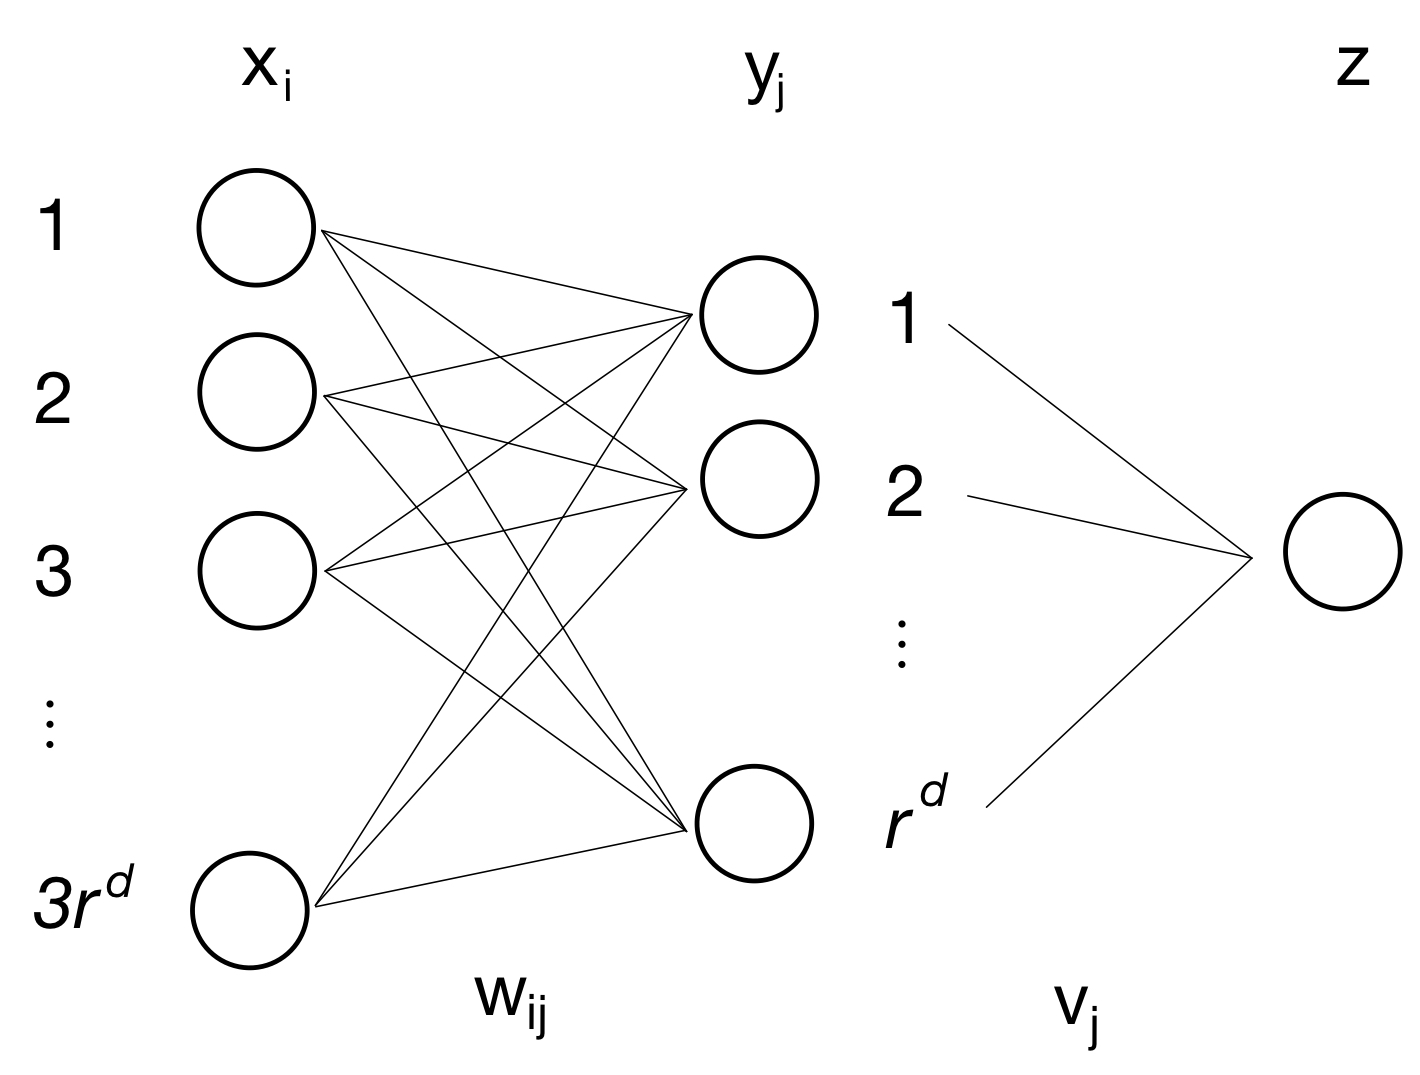
\includegraphics[width=0.5\textwidth]{images/ann.jpg}
    \caption{Návrh neurónovej siete}
\end{figure}
Implementácia tejto neurónovej siete je bližšie popísaná v \autoref{subsec:dev-tools-for-ai}.

Pre potreby natrénovania umelých neurónových sietí boli použité simulácie náhodných hier.
Simulácie pozostávali z náhodného výberu políčok pre každého hráča.
Náhodný výber bol navyše zlepšený predpokladom, že hráči sa počas hry (najmä na plochách väčších rozmerov) snažia
prevažne znemožniť protihráčovi jeho výhru výberom takých políčok, ktoré sú blízko jeho predchádzajúcemu ťahu
(resp. predchádzajúcim ťahom).
Keďže piškvorky sú hra, ktorá sa hrá na pravouhlej ploche (resp. pravouhlom priestore) bolo možné pri výpočte
pravdepodobnosti výberu prvku použiť Manhattanskú vzdialenosť.
Nech pre $d=3$ $c_i(b)$, $c_j(b)$, $c_k(b)$ sú súradnice ($i$, $j$ a $k$) políčka, ktoré je najbližšie k políčku
$b_{ijk}$ a nech
\begin{equation}
    e(b_{ijk}) =
    \begin{cases}
        1 & \text{ak políčko }ijk\text{ je prázdne} \\
        0 & \text{inak}
    \end{cases}
\end{equation}
potom pravdepodobnosť výberu políčka $ijk$ je
\begin{equation}
    p(b_{ijk}) = \frac{|c_i(b) - i| + |c_j(b) - j| + |c_k(b) - k|}{\sum_{m=1}^r\sum_{n=1}^r\sum_{o=1}^r e(b_{mno})}
\end{equation}
Pre $d=2$ (teda pre hru na ploche) platia rovnaké pravidlá, pričom $k=1$ (resp. $o=1$) vo všetkých prípadoch.

\subsection{Zisťovanie víťaza}\label{subsec:checking-winner}

Už kontrola víťaza pre plochu (2D priestor) s pevne danými rozmermi a pevne danou hodnotou počtu znakov potrebných pre
výhru (často zhodnou s rozmerom) je relatívne komplexná úloha.
Ak sú použité sofistikovanejšie prostriedky než fixný prístup k prvkom vektora prostredníctvom číselných indexov, tak
pre rozmer $r \times r$, kde $r = w$ má tento problém nasledovné riešenie:
\begin{lstlisting}[
  mathescape,
  columns=fullflexible,
  escapeinside={(@}{@)},
  basicstyle=\fontfamily{lmvtt}\selectfont,
]
pre $i=1\dots{r}$:
    ak $b_{i0}$ je (@pr\'{a}zdne@)
    inak:
        $z = b_{i0}$
        pre $j=1\dots{r}$:
            ak $b_{ij} \neq z$:
                (@prejdi na \v{d}al\v{s}\'{i} riadok@)
        (@v\'{i}\v{t}az je@) $z$
pre $j=1\dots{r}$:
    ak $b_{0j}$
    inak:
        $z = b_{0j}$
        pre $i=1\dots{r}$:
            ak $b_{ij} \neq z$:
                (@prejdi na \v{d}al\v{s}\'{i} st\'{l}pec@)
        (@v\'{i}\v{t}az je@) $z$
ak $b_{00}$ (@nie je pr\'{a}zdny znak@)
    $z = b_{00}$
    pre $i=1\dots{r}$:
        ak $b_{ii} \neq z$, koniec cyklu
    v\'{i}\v{t}az je $z$
ak $b_{0,r-i}$ (@nie je pr\'{a}zdny znak@)
    $z = b_{0,r-i}$
    pre $i=1\dots{r}$:
        ak $b_{i,r-i} \neq z$, koniec cyklu
    (@v\'{i}\v{t}az je@) $z$
(@ak \v{z}iadny z predo\v{s}l\'{y}ch cyklov nevyhodnot\'{i} v\'{i}\v{t}aza a@)
(@neexistuje \v{z}iaden mo\v{z}n\'{y} \v{t}ah pre hr\'{a}\v{c}a, nastala rem\'{i}za@)
\end{lstlisting}
Prvá a druhá časť skúmajú potenciálnych víťazov v riadku a stĺpci, druhá časť skúma výsledky diagonálne.
Keďže $r = w$ stačí preskúmať hlavnú a vedľajšiu diagonálu, pretože tie sú jediné, ktoré môžu obsahovať $w$ znakov.
Zložitosť tohto algoritmu je exponenciálna:
\begin{equation}
    \mathcal{O}(r.r + r.r + 2r + 2r) \sim \mathcal{O}(2r^2 + 4r) \sim \mathcal{O}(r^2)
\end{equation}

Nech $R$ je množina potenciálnych víťazných množín $M$ ($|M|=r$).
Algoritmus je možné prepísať nasledovne:
\begin{lstlisting}[
  mathescape,
  columns=fullflexible,
  escapeinside={(@}{@)},
  basicstyle=\fontfamily{lmvtt}\selectfont,
]
$R=\{\}$
$M_h=\{\}$
$M_v=\{\}$
pre $i=1\dots{r}$:
    $M_r=\{b_{ij}|j=1 \dots r\}$
    pridanie $M_r$ do $R$
    $M_s=\{b_{ji}|j=1 \dots r\}$
    pridanie $M_s$ do $R$
    pridanie $b_{ii}$ do $M_h$
    pridanie $b_{i,r-i}$ do $M_v$

pridanie $M_h$ do $R$
pridanie $M_v$ do $R$

pre $k=1\dots{|R|}$:
    $z$ = $k$-ty prvok z $R$
    pre $i=1\dots{r}$:
        ak $z_0 = z_i$, (@potom $z_0$ je v\'{i}\v{t}az@)
(@ak predo\v{s}l\'{y} cyklus nevyhodnot\'{i} v\'{i}\v{t}aza a@)
(@neexistuje \v{z}iaden mo\v{z}n\'{y} \v{t}ah pre hr\'{a}\v{c}a, nastala rem\'{i}za@)
\end{lstlisting}
Algoritmus najskôr vytvorí množinu $R$ z každého stĺpca a riadku ($M_r$ a $M_s$) a postupne plní množiny hlavnej a
vedľajšej diagonály ($M_h$ a $M_s$).
Za predpokladu, že $R$ je reprezentovaná štruktúrou, kde zložitosť vloženia je $\mathcal{O}(1)$ a
$|R| = r + r + 2 = 2r + 2$, potom celková zložitosť je znova exponenciálna, no algoritmus je omnoho kratší
\begin{equation}
    \mathcal{O}(r.2r + r.|R|) \sim \mathcal{O}(r.2r + r.(2r + 2)) \sim \mathcal{O}(2r^2 + 2r^2 + 2r) \sim \mathcal{O}(4r^2 + 2r) \sim \mathcal{O}(r^2)
\end{equation}

Takýto algoritmus je celkom jednoduchý a má prijateľnú (exponenciálnu) zložitosť vzhľadom na rozmer hracej plochy.
V prípade, že $r \neq w$, je nutné algoritmus rozšíriť.
Jeden zo spôsobov je taký, že vždy sa kontroluje iba plocha o veľkosti $w \times w$ (vyššie popísaným algoritmom) s
tým, že kontrolovaná plocha $W$ začína na počiatočných súradniciach $[x,y]=[1,1]$ a postupne sa súradnice zvyšujú o 1
tak, aby boli skontrolované všetky kombinácie počiatočných súradníc.
Počiatočné súradnice $x$ a $y$ nadobúdajú hodnoty z $C = \{1, 2, \dots, r - w\}$.
Algoritmus je možné upraviť nasledovne:
\begin{lstlisting}[
  mathescape,
  columns=fullflexible,
  escapeinside={(@}{@)},
  basicstyle=\fontfamily{lmvtt}\selectfont,
]
Nech $skontroluj(x, y)$:
    $R=\{\}$
    $M_h=\{\}$
    $M_v=\{\}$
    pre $i=x\dots{x + w}$:
        $M_r=\{b_{ij}|j=y \dots y + w\}$
        pridanie $M_r$ do $R$
        $M_s=\{b_{ji}|j=y \dots y + w\}$
        pridanie $M_s$ do $R$
        pridanie $b_{ii}$ do $M_h$
        pridanie $b_{i,r-i}$ do $M_v$

    pridanie $M_h$ do $R$
    pridanie $M_v$ do $R$

    pre $k=1\dots{|R|}$:
        $z$ = $k$-ty prvok z $R$
        pre $i=1\dots{w}$:
            ak $z_0 = z_i$, potom $z_0$ (@je v\'{i}\v{t}az@)
    (@ak predo\v{s}l\'{y} cyklus nevyhodnot\'{i} v\'{i}\v{t}aza tak@):
        ak $[x + 1, y]$ (@nebolo skontrolovan\'{e}@) $skontroluj(x + 1, y)$
        ak $[x, y + 1]$ (@nebolo skontrolovan\'{e}@) $skontroluj(x, y + 1)$
        ak $[x + 1, y + 1]$ (@nebolo skontrolovan\'{e}@) $skontroluj(x + 1, y + 1)$

$skontroluj(0, 0)$
\end{lstlisting}
Keďže procedúra $skontroluj$ je volaná vnútri jej definície, je jasné, že táto procedúra je \emph{rekurzívna}.
Nech $c = |C| = r - w$, potom počet volaní $skontroluj$ je $c$ a ak zložitosť procedúry $skontroluj(x, y)$ je
$\mathcal{O}(4r^2 + 2r)$, potom celková zložitosť je
\begin{equation}
    \mathcal{O}((4r^2 + 2r).c^2) \sim \mathcal{O}(4r^2c^2 + 2rc^2) \sim \mathcal{O}(r^2c^2)
\end{equation}

\begin{figure}[H]
    \centering
    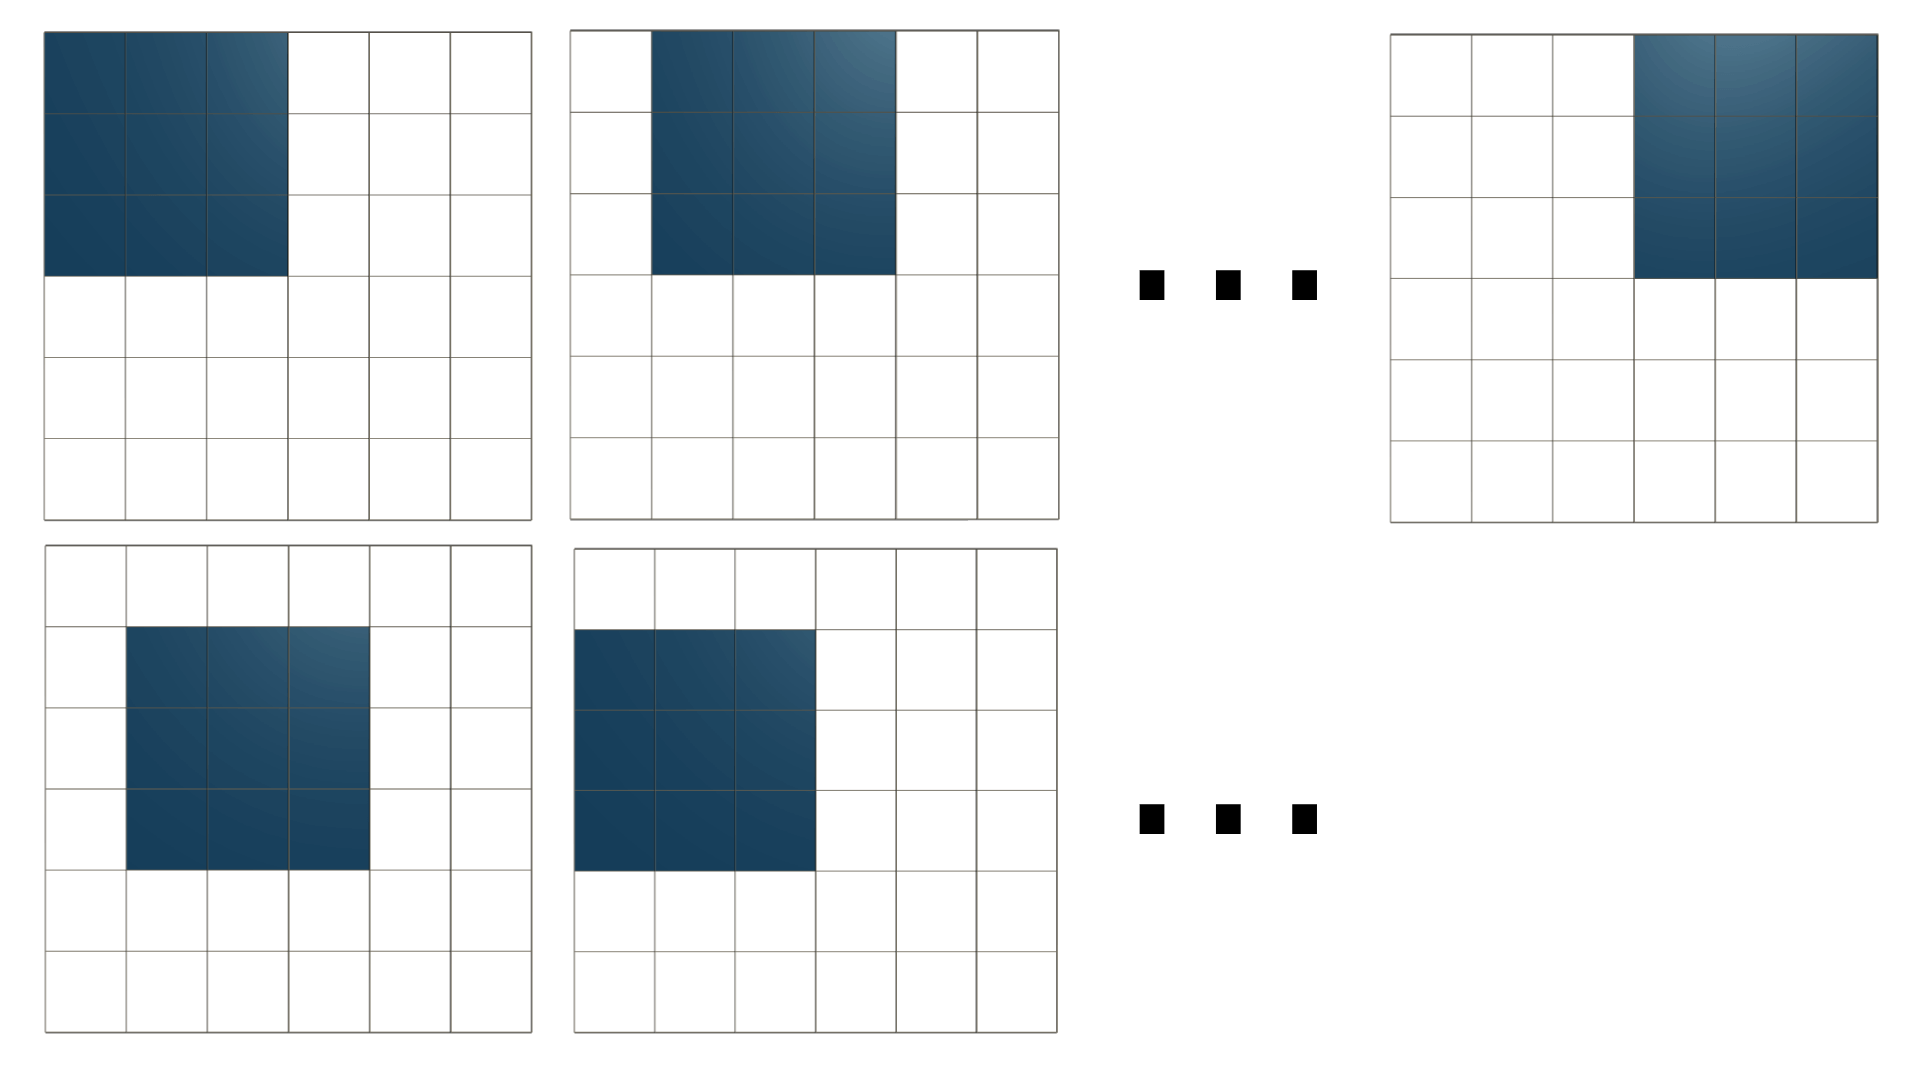
\includegraphics[width=1\textwidth]{images/winner-2D.png}
    \caption{Zisťovanie víťaza v 2D priestore}
\end{figure}

Analogicky je definovaný algoritmus pre tretí rozmer s pridanou kontrolou znakov v priestorových diagonálach, no
z dôvodu pridania jedného rozmeru (resp. $r$ plôch za sebou) je nutné tento princíp použiť na všetky 3 rozmery.
Zložitosť kontroly plochy $w \times w \times w$ tým pádom narastie až na $\mathcal{O}(r^3)$ a celková zložitosť až na
$\mathcal{O}(r^3c^3)$.

\begin{figure}[H]
    \centering
    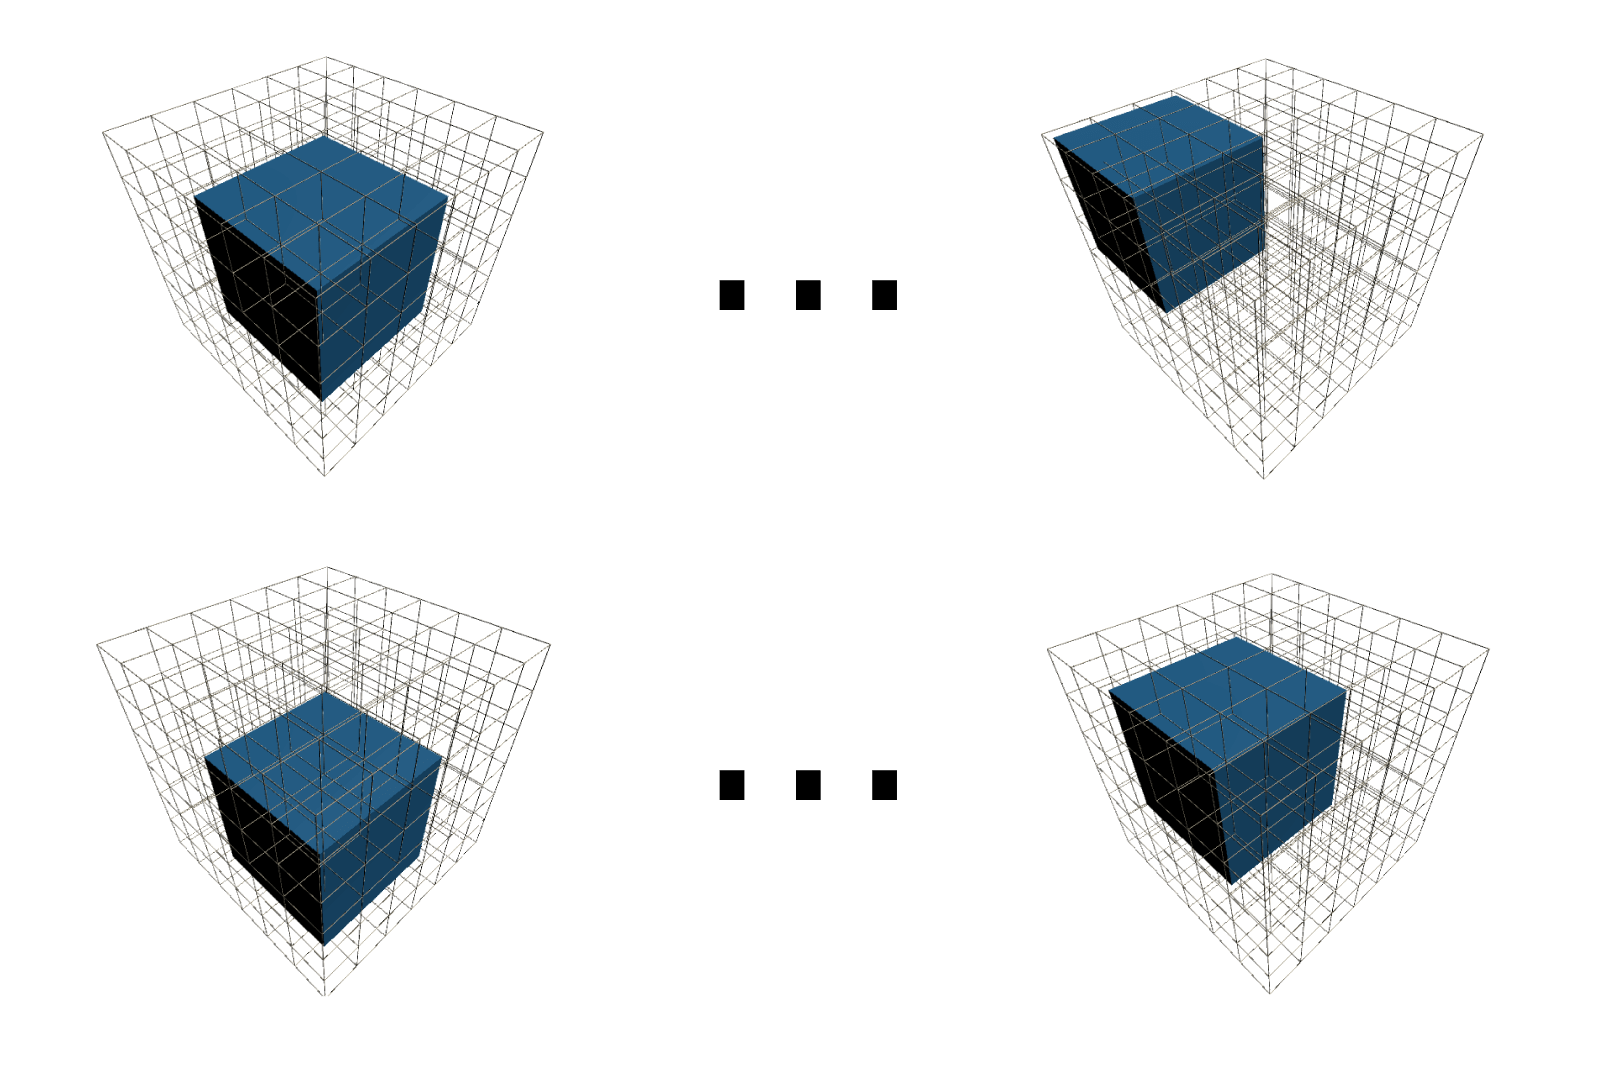
\includegraphics[width=0.8\textwidth]{images/winner-3D.png}
    \caption{Zisťovanie víťaza v 3D priestore}
\end{figure}

Zvolené algoritmy MiniMax a umelé neurónové siete majú obidva svoje výhody aj nevýhody.
Medzi základné výhody minimax-u patrí jeho optimálnosť.
Keďže táto metóda je exaktná, výsledok z tejto metódy je vždy zaručene optimálny no z tejto vlastnosti vyplýva aj to,
že prehľadáva celý priestor riešení a tým pádom je časovo neefektívny.
Na druhú stranu umelé neurónové siete sú oproti minimax-u veľmi rýchle a uberá im to zo správnosti ich riešení, no
len vo veľmi malej miere.
Vypísaný algoritmus na nájdenie víťaza je vzhľadom na vyhľadávací priestor relatívne efektívny.